\documentclass[]{article}
\usepackage{lmodern}
\usepackage{amssymb,amsmath}
\usepackage{ifxetex,ifluatex}
\usepackage{fixltx2e} % provides \textsubscript
\ifnum 0\ifxetex 1\fi\ifluatex 1\fi=0 % if pdftex
  \usepackage[T1]{fontenc}
  \usepackage[utf8]{inputenc}
\else % if luatex or xelatex
  \ifxetex
    \usepackage{mathspec}
  \else
    \usepackage{fontspec}
  \fi
  \defaultfontfeatures{Ligatures=TeX,Scale=MatchLowercase}
\fi
% use upquote if available, for straight quotes in verbatim environments
\IfFileExists{upquote.sty}{\usepackage{upquote}}{}
% use microtype if available
\IfFileExists{microtype.sty}{%
\usepackage{microtype}
\UseMicrotypeSet[protrusion]{basicmath} % disable protrusion for tt fonts
}{}
\usepackage[margin=1in]{geometry}
\usepackage{hyperref}
\hypersetup{unicode=true,
            pdftitle={HarranPlain},
            pdfauthor={Nicole Grunert},
            pdfborder={0 0 0},
            breaklinks=true}
\urlstyle{same}  % don't use monospace font for urls
\usepackage{color}
\usepackage{fancyvrb}
\newcommand{\VerbBar}{|}
\newcommand{\VERB}{\Verb[commandchars=\\\{\}]}
\DefineVerbatimEnvironment{Highlighting}{Verbatim}{commandchars=\\\{\}}
% Add ',fontsize=\small' for more characters per line
\usepackage{framed}
\definecolor{shadecolor}{RGB}{248,248,248}
\newenvironment{Shaded}{\begin{snugshade}}{\end{snugshade}}
\newcommand{\KeywordTok}[1]{\textcolor[rgb]{0.13,0.29,0.53}{\textbf{{#1}}}}
\newcommand{\DataTypeTok}[1]{\textcolor[rgb]{0.13,0.29,0.53}{{#1}}}
\newcommand{\DecValTok}[1]{\textcolor[rgb]{0.00,0.00,0.81}{{#1}}}
\newcommand{\BaseNTok}[1]{\textcolor[rgb]{0.00,0.00,0.81}{{#1}}}
\newcommand{\FloatTok}[1]{\textcolor[rgb]{0.00,0.00,0.81}{{#1}}}
\newcommand{\ConstantTok}[1]{\textcolor[rgb]{0.00,0.00,0.00}{{#1}}}
\newcommand{\CharTok}[1]{\textcolor[rgb]{0.31,0.60,0.02}{{#1}}}
\newcommand{\SpecialCharTok}[1]{\textcolor[rgb]{0.00,0.00,0.00}{{#1}}}
\newcommand{\StringTok}[1]{\textcolor[rgb]{0.31,0.60,0.02}{{#1}}}
\newcommand{\VerbatimStringTok}[1]{\textcolor[rgb]{0.31,0.60,0.02}{{#1}}}
\newcommand{\SpecialStringTok}[1]{\textcolor[rgb]{0.31,0.60,0.02}{{#1}}}
\newcommand{\ImportTok}[1]{{#1}}
\newcommand{\CommentTok}[1]{\textcolor[rgb]{0.56,0.35,0.01}{\textit{{#1}}}}
\newcommand{\DocumentationTok}[1]{\textcolor[rgb]{0.56,0.35,0.01}{\textbf{\textit{{#1}}}}}
\newcommand{\AnnotationTok}[1]{\textcolor[rgb]{0.56,0.35,0.01}{\textbf{\textit{{#1}}}}}
\newcommand{\CommentVarTok}[1]{\textcolor[rgb]{0.56,0.35,0.01}{\textbf{\textit{{#1}}}}}
\newcommand{\OtherTok}[1]{\textcolor[rgb]{0.56,0.35,0.01}{{#1}}}
\newcommand{\FunctionTok}[1]{\textcolor[rgb]{0.00,0.00,0.00}{{#1}}}
\newcommand{\VariableTok}[1]{\textcolor[rgb]{0.00,0.00,0.00}{{#1}}}
\newcommand{\ControlFlowTok}[1]{\textcolor[rgb]{0.13,0.29,0.53}{\textbf{{#1}}}}
\newcommand{\OperatorTok}[1]{\textcolor[rgb]{0.81,0.36,0.00}{\textbf{{#1}}}}
\newcommand{\BuiltInTok}[1]{{#1}}
\newcommand{\ExtensionTok}[1]{{#1}}
\newcommand{\PreprocessorTok}[1]{\textcolor[rgb]{0.56,0.35,0.01}{\textit{{#1}}}}
\newcommand{\AttributeTok}[1]{\textcolor[rgb]{0.77,0.63,0.00}{{#1}}}
\newcommand{\RegionMarkerTok}[1]{{#1}}
\newcommand{\InformationTok}[1]{\textcolor[rgb]{0.56,0.35,0.01}{\textbf{\textit{{#1}}}}}
\newcommand{\WarningTok}[1]{\textcolor[rgb]{0.56,0.35,0.01}{\textbf{\textit{{#1}}}}}
\newcommand{\AlertTok}[1]{\textcolor[rgb]{0.94,0.16,0.16}{{#1}}}
\newcommand{\ErrorTok}[1]{\textcolor[rgb]{0.64,0.00,0.00}{\textbf{{#1}}}}
\newcommand{\NormalTok}[1]{{#1}}
\usepackage{longtable,booktabs}
\usepackage{graphicx,grffile}
\makeatletter
\def\maxwidth{\ifdim\Gin@nat@width>\linewidth\linewidth\else\Gin@nat@width\fi}
\def\maxheight{\ifdim\Gin@nat@height>\textheight\textheight\else\Gin@nat@height\fi}
\makeatother
% Scale images if necessary, so that they will not overflow the page
% margins by default, and it is still possible to overwrite the defaults
% using explicit options in \includegraphics[width, height, ...]{}
\setkeys{Gin}{width=\maxwidth,height=\maxheight,keepaspectratio}
\IfFileExists{parskip.sty}{%
\usepackage{parskip}
}{% else
\setlength{\parindent}{0pt}
\setlength{\parskip}{6pt plus 2pt minus 1pt}
}
\setlength{\emergencystretch}{3em}  % prevent overfull lines
\providecommand{\tightlist}{%
  \setlength{\itemsep}{0pt}\setlength{\parskip}{0pt}}
\setcounter{secnumdepth}{5}
% Redefines (sub)paragraphs to behave more like sections
\ifx\paragraph\undefined\else
\let\oldparagraph\paragraph
\renewcommand{\paragraph}[1]{\oldparagraph{#1}\mbox{}}
\fi
\ifx\subparagraph\undefined\else
\let\oldsubparagraph\subparagraph
\renewcommand{\subparagraph}[1]{\oldsubparagraph{#1}\mbox{}}
\fi

%%% Use protect on footnotes to avoid problems with footnotes in titles
\let\rmarkdownfootnote\footnote%
\def\footnote{\protect\rmarkdownfootnote}

%%% Change title format to be more compact
\usepackage{titling}

% Create subtitle command for use in maketitle
\newcommand{\subtitle}[1]{
  \posttitle{
    \begin{center}\large#1\end{center}
    }
}

\setlength{\droptitle}{-2em}
  \title{HarranPlain}
  \pretitle{\vspace{\droptitle}\centering\huge}
  \posttitle{\par}
  \author{Nicole Grunert}
  \preauthor{\centering\large\emph}
  \postauthor{\par}
  \predate{\centering\large\emph}
  \postdate{\par}
  \date{20 Juli 2017}


\begin{document}
\maketitle

{
\setcounter{tocdepth}{2}
\tableofcontents
}
\begin{Shaded}
\begin{Highlighting}[]
\NormalTok{knitr::opts_chunk$}\KeywordTok{set}\NormalTok{(}\DataTypeTok{echo =} \OtherTok{TRUE}\NormalTok{) }\CommentTok{#include=FALSE nicht in pdf output?}
\end{Highlighting}
\end{Shaded}

\subsection{Point Pattern}\label{point-pattern}

\begin{Shaded}
\begin{Highlighting}[]
\NormalTok{harran=}\KeywordTok{read.table}\NormalTok{(}\StringTok{"../data/Sites_HarranPlain.csv"}\NormalTok{,}
                  \DataTypeTok{sep =} \StringTok{","}\NormalTok{,}
                  \DataTypeTok{header =} \OtherTok{TRUE}\NormalTok{)   }\CommentTok{# when knitting: "../data/Sites_HarranPlain.csv"!!!!!}
\KeywordTok{str}\NormalTok{(harran)}
\end{Highlighting}
\end{Shaded}

\begin{verbatim}
## 'data.frame':    344 obs. of  5 variables:
##  $ X.1            : int  1 2 3 4 5 6 7 8 9 10 ...
##  $ Name           : Factor w/ 166 levels "Ömertepe","Öncül (FALSCH)",..: 24 10 10 67 67 67 67 78 78 78 ...
##  $ X              : num  38.8 38.9 38.9 38.9 38.9 ...
##  $ Y              : num  37.6 37.7 37.7 37.2 37.2 ...
##  $ Mentioned_Epoch: Factor w/ 179 levels "","-","Aceramic Neolithic ",..: 175 150 139 162 108 151 161 134 125 86 ...
\end{verbatim}

\subsection{spatstat}\label{spatstat}

\begin{Shaded}
\begin{Highlighting}[]
\KeywordTok{library}\NormalTok{(sp)}
\end{Highlighting}
\end{Shaded}

\begin{verbatim}
## Warning: package 'sp' was built under R version 3.3.3
\end{verbatim}

\begin{Shaded}
\begin{Highlighting}[]
\KeywordTok{coordinates}\NormalTok{(harran) <-}\StringTok{ }\ErrorTok{~}\NormalTok{X+Y}
\KeywordTok{proj4string}\NormalTok{(harran) <-}\StringTok{ }\KeywordTok{CRS}\NormalTok{(}\StringTok{"+init=epsg:4326"}\NormalTok{)}

\NormalTok{harran <-}\StringTok{ }\KeywordTok{spTransform}\NormalTok{(harran, }\DataTypeTok{CRSobj =} \KeywordTok{CRS}\NormalTok{(}\StringTok{"+init=epsg:32637"}\NormalTok{))}
\KeywordTok{str}\NormalTok{(harran) }\CommentTok{# for checking}
\end{Highlighting}
\end{Shaded}

\begin{verbatim}
## Formal class 'SpatialPointsDataFrame' [package "sp"] with 5 slots
##   ..@ data       :'data.frame':  344 obs. of  3 variables:
##   .. ..$ X.1            : int [1:344] 1 2 3 4 5 6 7 8 9 10 ...
##   .. ..$ Name           : Factor w/ 166 levels "Ömertepe","Öncül (FALSCH)",..: 24 10 10 67 67 67 67 78 78 78 ...
##   .. ..$ Mentioned_Epoch: Factor w/ 179 levels "","-","Aceramic Neolithic ",..: 175 150 139 162 108 151 161 134 125 86 ...
##   ..@ coords.nrs : num(0) 
##   ..@ coords     : num [1:344, 1:2] 479412 486771 486771 493122 493122 ...
##   .. ..- attr(*, "dimnames")=List of 2
##   .. .. ..$ : chr [1:344] "1" "2" "3" "4" ...
##   .. .. ..$ : chr [1:2] "X" "Y"
##   ..@ bbox       : num [1:2, 1:2] 477942 4062337 514430 4290885
##   .. ..- attr(*, "dimnames")=List of 2
##   .. .. ..$ : chr [1:2] "X" "Y"
##   .. .. ..$ : chr [1:2] "min" "max"
##   ..@ proj4string:Formal class 'CRS' [package "sp"] with 1 slot
##   .. .. ..@ projargs: chr "+init=epsg:32637 +proj=utm +zone=37 +datum=WGS84 +units=m +no_defs +ellps=WGS84 +towgs84=0,0,0"
\end{verbatim}

\begin{Shaded}
\begin{Highlighting}[]
\KeywordTok{library}\NormalTok{(spatstat)}
\end{Highlighting}
\end{Shaded}

\begin{verbatim}
## Warning: package 'spatstat' was built under R version 3.3.3
\end{verbatim}

\begin{verbatim}
## Loading required package: nlme
\end{verbatim}

\begin{verbatim}
## Warning: package 'nlme' was built under R version 3.3.3
\end{verbatim}

\begin{verbatim}
## Loading required package: rpart
\end{verbatim}

\begin{verbatim}
## Warning: package 'rpart' was built under R version 3.3.3
\end{verbatim}

\begin{verbatim}
## 
## spatstat 1.51-0       (nickname: 'Poetic Licence') 
## For an introduction to spatstat, type 'beginner'
\end{verbatim}

\begin{verbatim}
## 
## Note: R version 3.3.1 (2016-06-21) is more than 9 months old; we strongly recommend upgrading to the latest version
\end{verbatim}

\begin{Shaded}
\begin{Highlighting}[]
\KeywordTok{str}\NormalTok{(harran@coords) }\CommentTok{# structure}
\end{Highlighting}
\end{Shaded}

\begin{verbatim}
##  num [1:344, 1:2] 479412 486771 486771 493122 493122 ...
##  - attr(*, "dimnames")=List of 2
##   ..$ : chr [1:344] "1" "2" "3" "4" ...
##   ..$ : chr [1:2] "X" "Y"
\end{verbatim}

\begin{Shaded}
\begin{Highlighting}[]
\NormalTok{harran_ppp <-}\StringTok{ }\KeywordTok{ppp}\NormalTok{(}\DataTypeTok{x=}\NormalTok{harran@coords[,}\DecValTok{1}\NormalTok{],}
                  \DataTypeTok{y=}\NormalTok{harran@coords[,}\DecValTok{2}\NormalTok{],}
                  \DataTypeTok{window =} \KeywordTok{owin}\NormalTok{(}\DataTypeTok{xrange =} \NormalTok{harran@bbox[}\DecValTok{1}\NormalTok{,],}
                                \DataTypeTok{yrange =} \KeywordTok{c}\NormalTok{(}\KeywordTok{min}\NormalTok{(harran@coords[,}\DecValTok{2}\NormalTok{]),}
                                           \KeywordTok{min}\NormalTok{(harran@coords[,}\DecValTok{2}\NormalTok{])+}\DecValTok{52000}\NormalTok{)))}
\end{Highlighting}
\end{Shaded}

\begin{verbatim}
## Warning: 65 points were rejected as lying outside the specified window
\end{verbatim}

\begin{verbatim}
## Warning: data contain duplicated points
\end{verbatim}

\begin{Shaded}
\begin{Highlighting}[]
\NormalTok{harran_ppp=}\KeywordTok{unique.ppp}\NormalTok{(harran_ppp) }\CommentTok{# shows number of duplicated points and deletes them/ harran_ppp= has to be done to define harran_ppp new}

\KeywordTok{str}\NormalTok{(harran_ppp)}
\end{Highlighting}
\end{Shaded}

\begin{verbatim}
## List of 5
##  $ window    :List of 4
##   ..$ type  : chr "rectangle"
##   ..$ xrange: Named num [1:2] 477942 514430
##   .. ..- attr(*, "names")= chr [1:2] "min" "max"
##   ..$ yrange: num [1:2] 4062337 4114337
##   ..$ units :List of 3
##   .. ..$ singular  : chr "unit"
##   .. ..$ plural    : chr "units"
##   .. ..$ multiplier: num 1
##   .. ..- attr(*, "class")= chr "units"
##   ..- attr(*, "class")= chr "owin"
##  $ n         : int 149
##  $ x         : num [1:149] 485197 491077 482518 497239 495545 ...
##  $ y         : num [1:149] 4109677 4070842 4104300 4083259 4083780 ...
##  $ markformat: chr "none"
##  - attr(*, "class")= chr "ppp"
\end{verbatim}

\begin{Shaded}
\begin{Highlighting}[]
\KeywordTok{plot}\NormalTok{(harran_ppp)}
\end{Highlighting}
\end{Shaded}

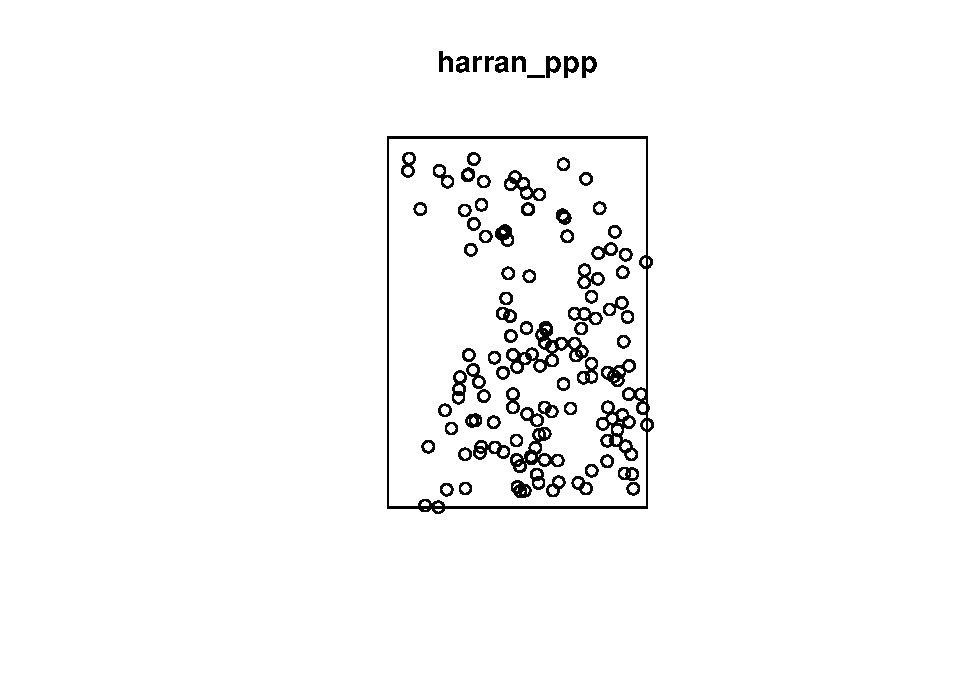
\includegraphics{HarranPlain_files/figure-latex/unnamed-chunk-2-1.pdf}

\begin{Shaded}
\begin{Highlighting}[]
\KeywordTok{library}\NormalTok{(mapview)}
\end{Highlighting}
\end{Shaded}

\begin{verbatim}
## Warning: package 'mapview' was built under R version 3.3.3
\end{verbatim}

\begin{verbatim}
## Loading required package: leaflet
\end{verbatim}

\begin{verbatim}
## Warning: package 'leaflet' was built under R version 3.3.3
\end{verbatim}

\begin{Shaded}
\begin{Highlighting}[]
\KeywordTok{mapview}\NormalTok{(harran)}
\end{Highlighting}
\end{Shaded}

\includegraphics{HarranPlain_files/figure-latex/unnamed-chunk-2-2.pdf}

\subsection{Challenge: delete duplicated
points}\label{challenge-delete-duplicated-points}

\begin{Shaded}
\begin{Highlighting}[]
\NormalTok{harran_ppp=}\KeywordTok{unique.ppp}\NormalTok{(harran_ppp) }\CommentTok{# shows number of duplicated points and deletes them/ harran_ppp= has to be done to define harran_ppp new}


\CommentTok{# or:}
\CommentTok{#anyDuplicated(harran_ppp)}
\CommentTok{#harran <- unique(harran_ppp)}
\CommentTok{#harran_ppp <- harran_ppp[!duplicated(harran_ppp)]}

\KeywordTok{plot}\NormalTok{(harran_ppp)}
\end{Highlighting}
\end{Shaded}

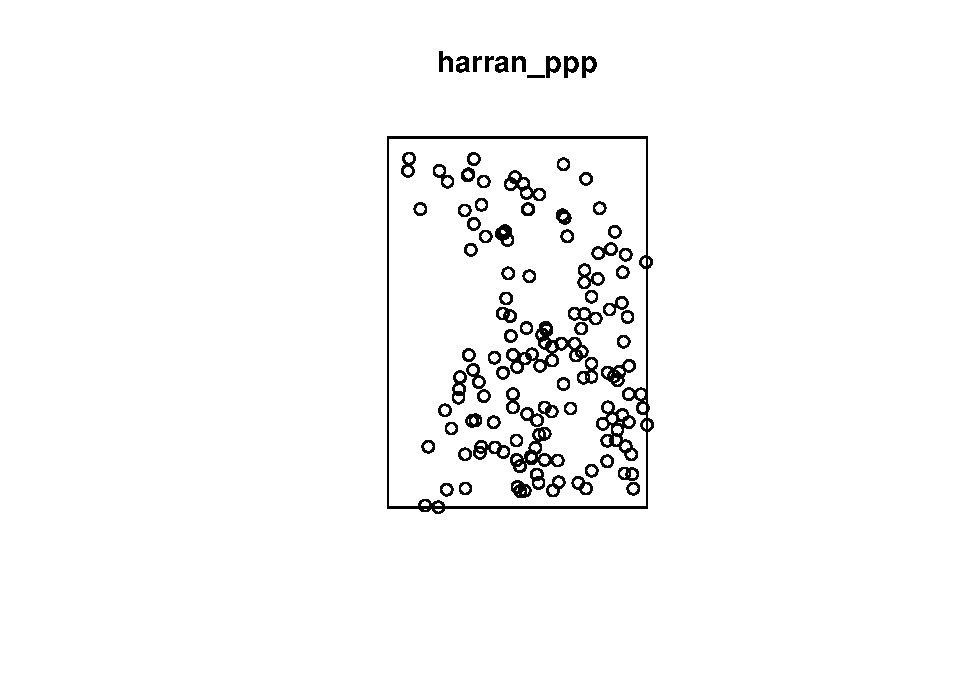
\includegraphics{HarranPlain_files/figure-latex/unnamed-chunk-3-1.pdf}

\section{Nearest neighbour distance}\label{nearest-neighbour-distance}

\begin{Shaded}
\begin{Highlighting}[]
\NormalTok{harran_ppp_nn <-}\StringTok{ }\KeywordTok{nndist}\NormalTok{(harran_ppp)}
\KeywordTok{str}\NormalTok{(harran_ppp_nn) }\CommentTok{# shows distance within the structure(str)}
\end{Highlighting}
\end{Shaded}

\begin{verbatim}
##  num [1:149] 1896 868 5436 1149 1772 ...
\end{verbatim}

\begin{Shaded}
\begin{Highlighting}[]
\KeywordTok{hist}\NormalTok{(harran_ppp_nn)  }\CommentTok{# plots the nearest neighbour}
\end{Highlighting}
\end{Shaded}

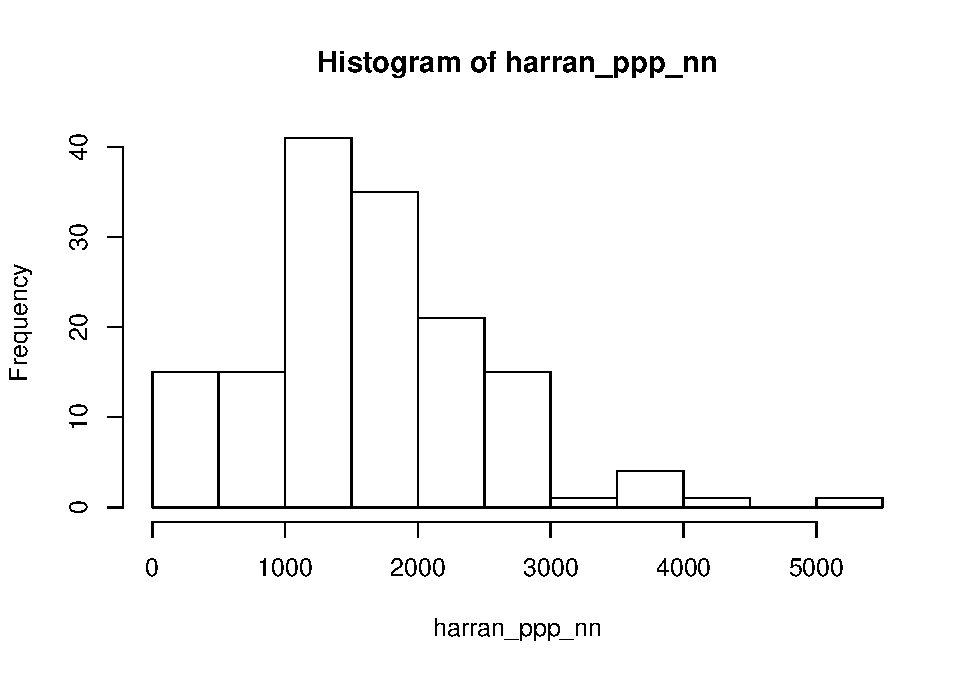
\includegraphics{HarranPlain_files/figure-latex/unnamed-chunk-4-1.pdf}

\begin{Shaded}
\begin{Highlighting}[]
\CommentTok{#barplot(sort(harran_ppp_nn))}
\end{Highlighting}
\end{Shaded}

\section{challenge: create a kernel density
estimation}\label{challenge-create-a-kernel-density-estimation}

\begin{Shaded}
\begin{Highlighting}[]
\NormalTok{harran_kde <-}\StringTok{ }\KeywordTok{density.ppp}\NormalTok{(harran_ppp,}\DataTypeTok{sigma =} \KeywordTok{mean}\NormalTok{(harran_ppp_nn))}\CommentTok{# see: likelihood cross validation bandwidth selection for kernel density (help)}
\KeywordTok{plot}\NormalTok{(harran_kde)}
\end{Highlighting}
\end{Shaded}

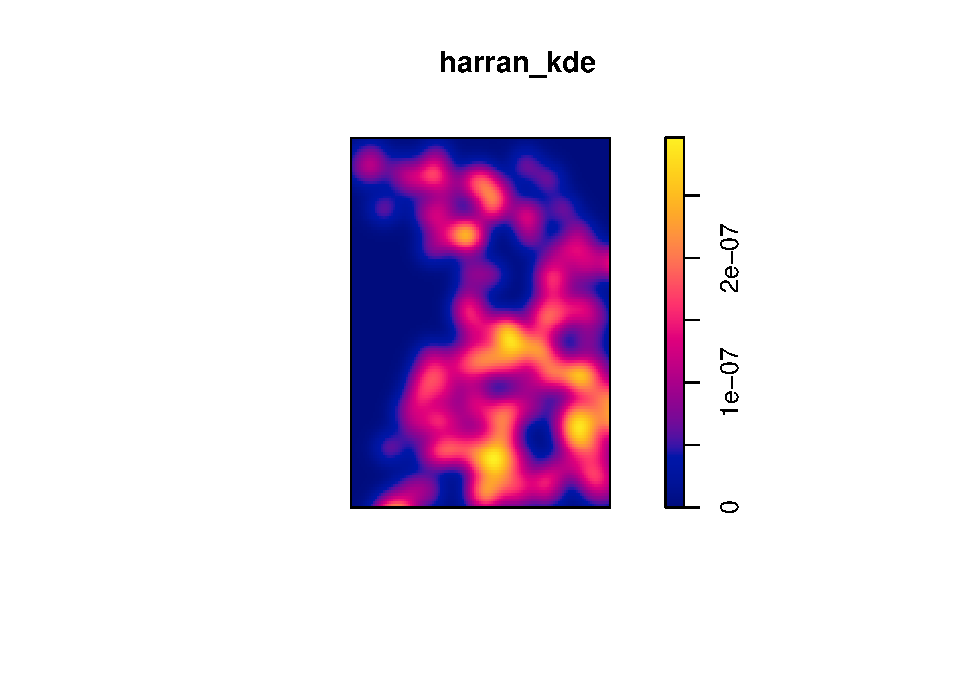
\includegraphics{HarranPlain_files/figure-latex/unnamed-chunk-5-1.pdf}

\section{raster}\label{raster}

\begin{Shaded}
\begin{Highlighting}[]
\KeywordTok{library}\NormalTok{(raster)}
\end{Highlighting}
\end{Shaded}

\begin{verbatim}
## Warning: package 'raster' was built under R version 3.3.3
\end{verbatim}

\begin{verbatim}
## 
## Attaching package: 'raster'
\end{verbatim}

\begin{verbatim}
## The following objects are masked from 'package:spatstat':
## 
##     area, rotate, shift
\end{verbatim}

\begin{verbatim}
## The following object is masked from 'package:nlme':
## 
##     getData
\end{verbatim}

\begin{Shaded}
\begin{Highlighting}[]
\NormalTok{dem <-}\StringTok{ }\KeywordTok{raster}\NormalTok{(}\StringTok{"../data/dem.tif"}\NormalTok{) }\CommentTok{# see above for problems when knitting}

\CommentTok{# or: library(rgdal)}
\CommentTok{#dem <- readGDAL("data/dem.tif")}
\KeywordTok{plot}\NormalTok{(dem)}
\end{Highlighting}
\end{Shaded}

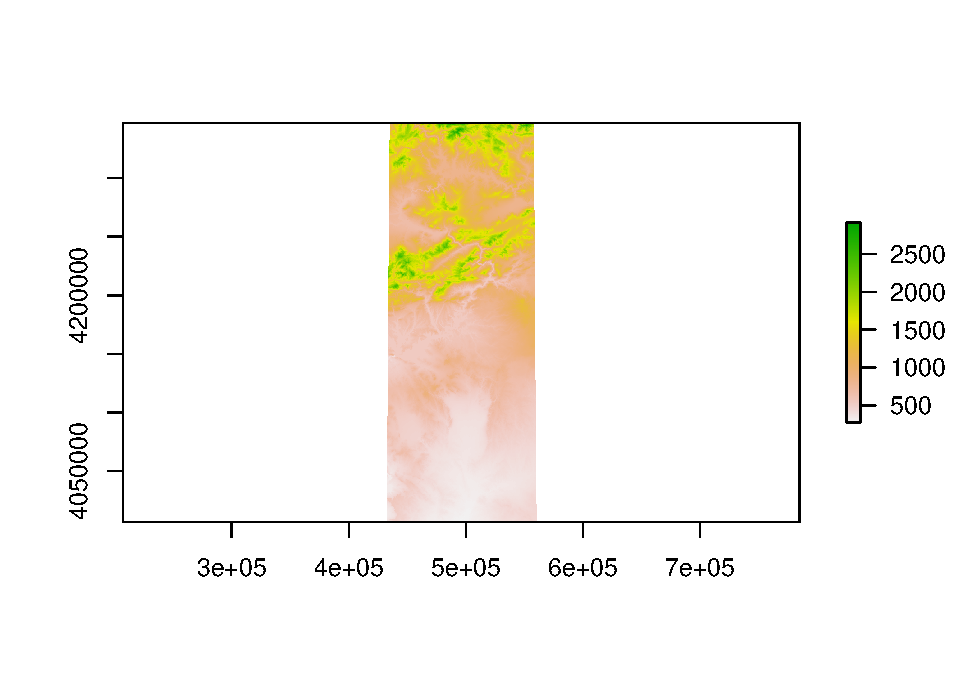
\includegraphics{HarranPlain_files/figure-latex/unnamed-chunk-6-1.pdf}

\begin{Shaded}
\begin{Highlighting}[]
\NormalTok{im_dem <-}\StringTok{ }\KeywordTok{as.im}\NormalTok{(}\KeywordTok{as.image.SpatialGridDataFrame}\NormalTok{(}\KeywordTok{as}\NormalTok{(dem,}\StringTok{"SpatialGridDataFrame"}\NormalTok{))) }\CommentTok{#creates image}
\KeywordTok{plot}\NormalTok{(im_dem)}
\end{Highlighting}
\end{Shaded}

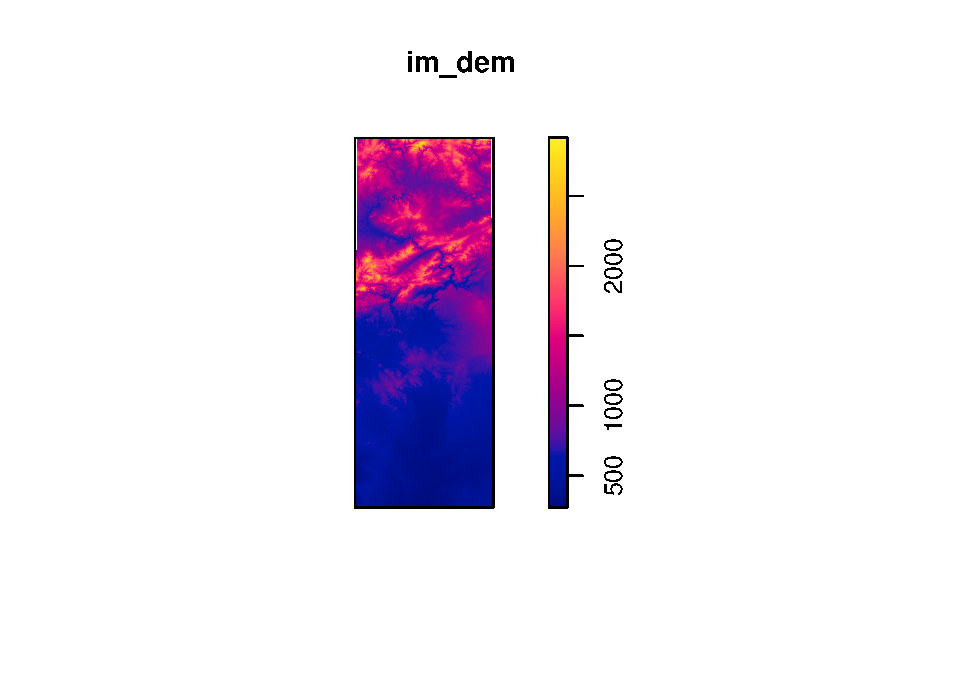
\includegraphics{HarranPlain_files/figure-latex/unnamed-chunk-6-2.pdf}

\section{challenge: use rhohat and create a
plot}\label{challenge-use-rhohat-and-create-a-plot}

\begin{Shaded}
\begin{Highlighting}[]
\CommentTok{#?rhohat # smoothing estimate: changes the raster}
\NormalTok{harran_rhohat <-}\StringTok{ }\KeywordTok{rhohat}\NormalTok{(harran_ppp,im_dem,}\DataTypeTok{bw =} \DecValTok{200}\NormalTok{)}
              \CommentTok{# <- rhohat(harran_ppp, im_dem, bw=200) /gives a more distinct picture}

\KeywordTok{plot}\NormalTok{(harran_rhohat) }\CommentTok{#x=elevation y=relative intensity of points -> relation of elevation to pointdensity, bandwidth=default -> default=sigma in the structure of the object(str(harran_rhohat))}
\end{Highlighting}
\end{Shaded}

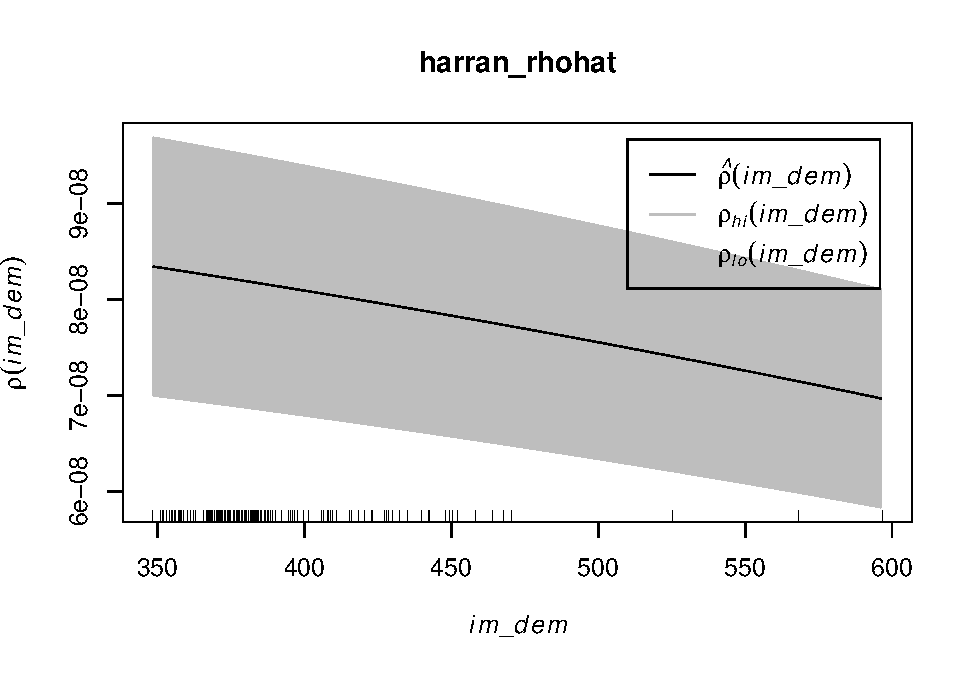
\includegraphics{HarranPlain_files/figure-latex/unnamed-chunk-7-1.pdf}

\begin{Shaded}
\begin{Highlighting}[]
\NormalTok{rho_dem <-}\StringTok{ }\KeywordTok{predict}\NormalTok{(harran_rhohat)}
\KeywordTok{plot}\NormalTok{(rho_dem)}
\end{Highlighting}
\end{Shaded}

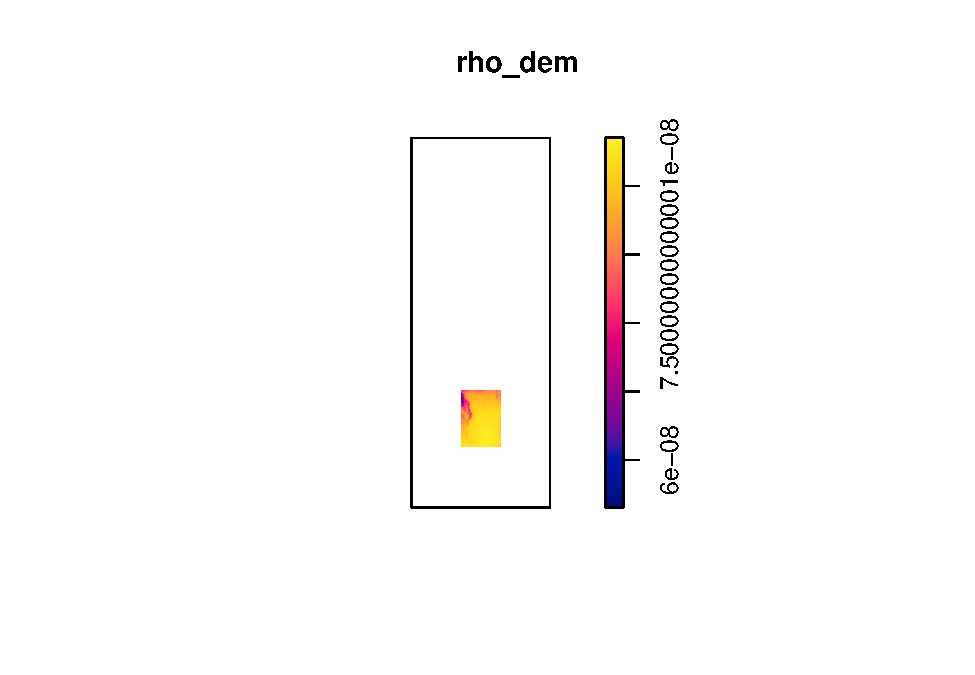
\includegraphics{HarranPlain_files/figure-latex/unnamed-chunk-7-2.pdf}

\begin{Shaded}
\begin{Highlighting}[]
\NormalTok{diff_rho <-}\StringTok{ }\NormalTok{harran_kde-rho_dem}
\end{Highlighting}
\end{Shaded}

\begin{verbatim}
## Warning: the images 'e1' and 'e2' were not compatible
\end{verbatim}

\begin{Shaded}
\begin{Highlighting}[]
\KeywordTok{plot}\NormalTok{(diff_rho)}
\end{Highlighting}
\end{Shaded}

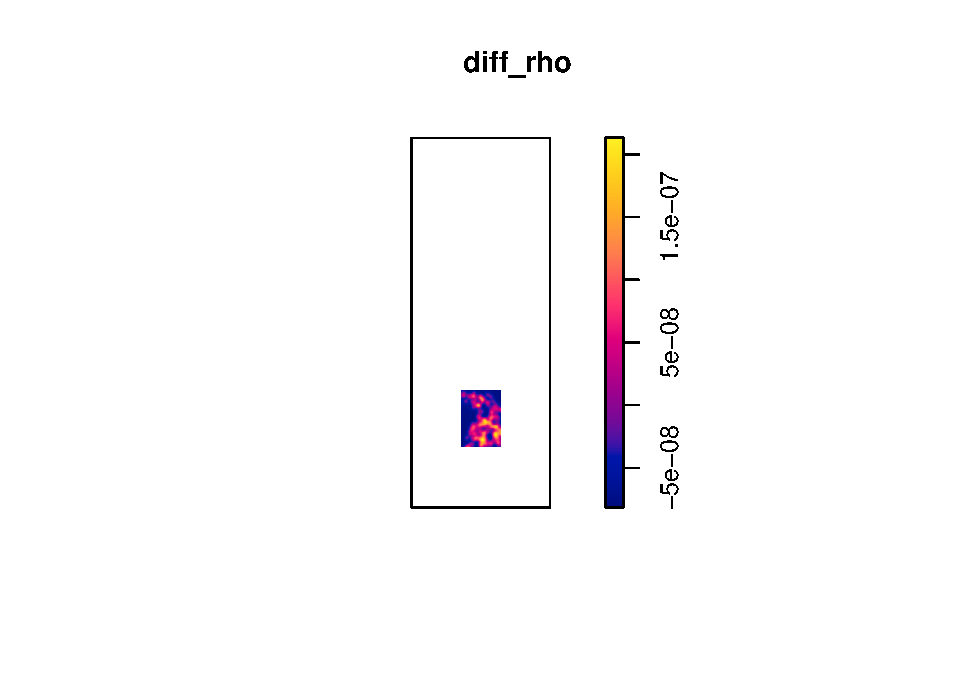
\includegraphics{HarranPlain_files/figure-latex/unnamed-chunk-7-3.pdf}

\section{challenge: test poisson, create random points with rpoispp
function that have the same intensity like our
points}\label{challenge-test-poisson-create-random-points-with-rpoispp-function-that-have-the-same-intensity-like-our-points}

\begin{Shaded}
\begin{Highlighting}[]
\KeywordTok{set.seed}\NormalTok{(}\DecValTok{123}\NormalTok{)}
\NormalTok{harran_rpoispp2 <-}\StringTok{ }\KeywordTok{rpoispp}\NormalTok{(}\DataTypeTok{lambda =} \NormalTok{harran_ppp$n/}\KeywordTok{area.owin}\NormalTok{(harran_ppp$window), }\DataTypeTok{win=}\NormalTok{harran_ppp$window)}
\KeywordTok{set.seed}\NormalTok{(}\DecValTok{123}\NormalTok{)}
\NormalTok{harran_rpoispp3 <-}\StringTok{ }\KeywordTok{rpoispp}\NormalTok{(}\KeywordTok{intensity}\NormalTok{(harran_ppp),}\DataTypeTok{win=}\KeywordTok{Window}\NormalTok{(harran_ppp))}
\KeywordTok{set.seed}\NormalTok{(}\DecValTok{123}\NormalTok{)}
\NormalTok{harran_rpoispp4 <-}\StringTok{ }\KeywordTok{rpoispp}\NormalTok{(}\DataTypeTok{ex =} \NormalTok{harran_ppp)}

\KeywordTok{plot}\NormalTok{(harran_ppp)}
\KeywordTok{points}\NormalTok{(harran_rpoispp2,}\DataTypeTok{col=}\StringTok{"green"}\NormalTok{)}
\KeywordTok{points}\NormalTok{(harran_rpoispp3,}\DataTypeTok{col=}\StringTok{"blue"}\NormalTok{)}
\KeywordTok{points}\NormalTok{(harran_rpoispp4,}\DataTypeTok{col=}\StringTok{"red"}\NormalTok{)}
\end{Highlighting}
\end{Shaded}

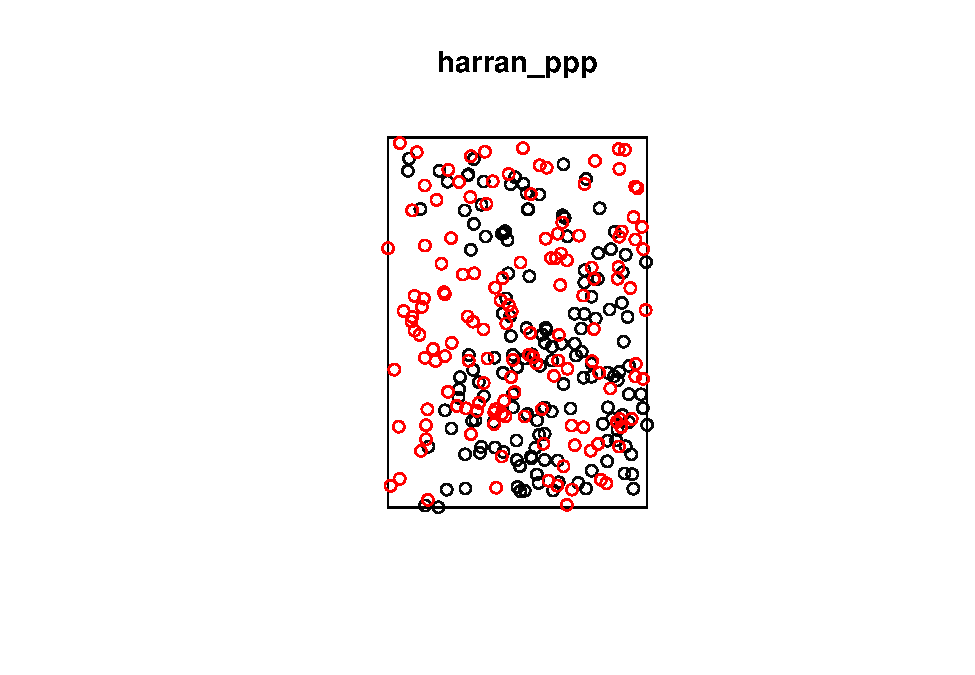
\includegraphics{HarranPlain_files/figure-latex/unnamed-chunk-8-1.pdf}

\begin{Shaded}
\begin{Highlighting}[]
\CommentTok{# first block is all the same, different ways to get the same result}
\end{Highlighting}
\end{Shaded}

\section{Second order effects}\label{second-order-effects}

\begin{Shaded}
\begin{Highlighting}[]
\NormalTok{harran_g <-}\StringTok{ }\KeywordTok{Gest}\NormalTok{(harran_ppp)}
\KeywordTok{str}\NormalTok{(harran_g)}
\end{Highlighting}
\end{Shaded}

\begin{verbatim}
## Classes 'fv' and 'data.frame':   513 obs. of  7 variables:
##  $ r      : num  0 13.3 26.7 40 53.4 ...
##  $ theo   : num  0.00 4.39e-05 1.76e-04 3.95e-04 7.02e-04 ...
##  $ han    : num  0 0 0 0 0 ...
##  $ rs     : num  0 0 0 0 0 ...
##  $ km     : num  0 0 0 0 0 ...
##  $ hazard : num  0 0 0 0 0 ...
##  $ theohaz: num  0.00 6.58e-06 1.32e-05 1.97e-05 2.63e-05 ...
##  - attr(*, "argu")= chr "r"
##  - attr(*, "valu")= chr "km"
##  - attr(*, "ylab")= language G(r)
##  - attr(*, "yexp")= language G(r)
##  - attr(*, "fmla")= chr ".~r"
##  - attr(*, "alim")= num  0 2628
##  - attr(*, "labl")= chr  "r" "%s[pois](r)" "hat(%s)[han](r)" "hat(%s)[bord](r)" ...
##  - attr(*, "desc")= chr  "distance argument r" "theoretical Poisson %s" "Hanisch estimate of %s" "border corrected estimate of %s" ...
##  - attr(*, "units")=List of 3
##   ..$ singular  : chr "unit"
##   ..$ plural    : chr "units"
##   ..$ multiplier: num 1
##   ..- attr(*, "class")= chr "units"
##  - attr(*, "fname")= chr "G"
##  - attr(*, "dotnames")= chr  "km" "rs" "han" "theo"
\end{verbatim}

\begin{Shaded}
\begin{Highlighting}[]
\KeywordTok{plot}\NormalTok{(harran_g) }\CommentTok{# x=closest neighbours expected (blue), the rest shows higher than expected clusters y= distance}
\end{Highlighting}
\end{Shaded}

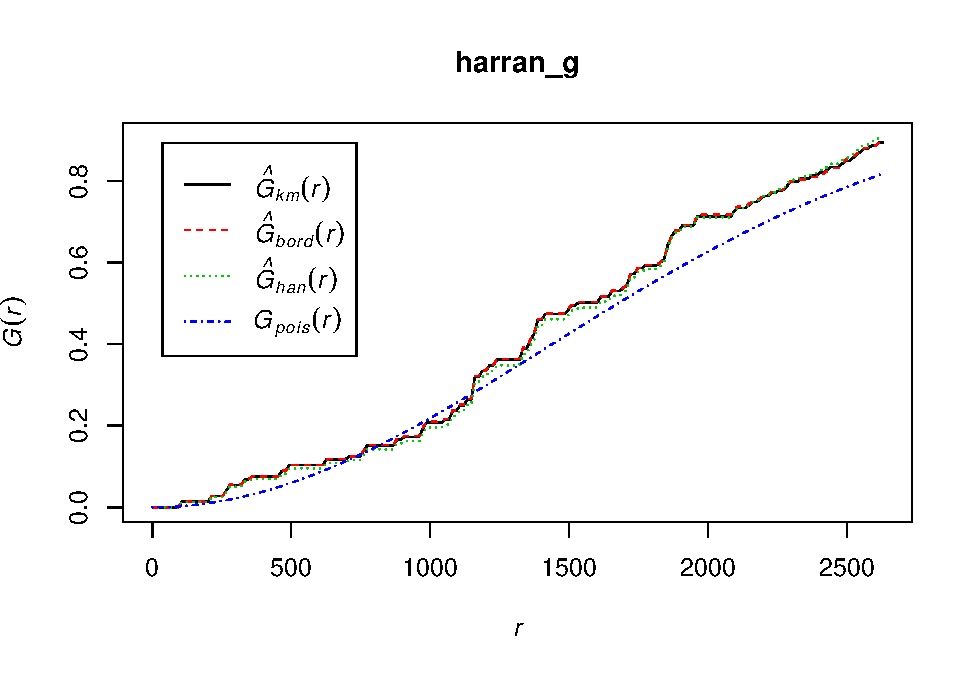
\includegraphics{HarranPlain_files/figure-latex/unnamed-chunk-9-1.pdf}

\begin{Shaded}
\begin{Highlighting}[]
\NormalTok{harran_ge <-}\StringTok{ }\KeywordTok{envelope}\NormalTok{(harran_ppp,}\DataTypeTok{fun =} \StringTok{"Gest"}\NormalTok{) }\CommentTok{# calculates g function for random points}
\end{Highlighting}
\end{Shaded}

\begin{verbatim}
## Generating 99 simulations of CSR  ...
## 1, 2, 3, 4, 5, 6, 7, 8, 9, 10, 11, 12, 13, 14, 15, 16, 17, 18, 19, 20, 21, 22, 23, 24, 25, 26, 27, 28, 29, 30, 31, 32, 33, 34, 35, 36, 37, 38,
## 39, 40, 41, 42, 43, 44, 45, 46, 47, 48, 49, 50, 51, 52, 53, 54, 55, 56, 57, 58, 59, 60, 61, 62, 63, 64, 65, 66, 67, 68, 69, 70, 71, 72, 73, 74, 75, 76,
## 77, 78, 79, 80, 81, 82, 83, 84, 85, 86, 87, 88, 89, 90, 91, 92, 93, 94, 95, 96, 97, 98,  99.
## 
## Done.
\end{verbatim}

\begin{Shaded}
\begin{Highlighting}[]
\KeywordTok{plot}\NormalTok{(harran_ge) }\CommentTok{# grey shadow_ monte Carlo Simulation}
\end{Highlighting}
\end{Shaded}

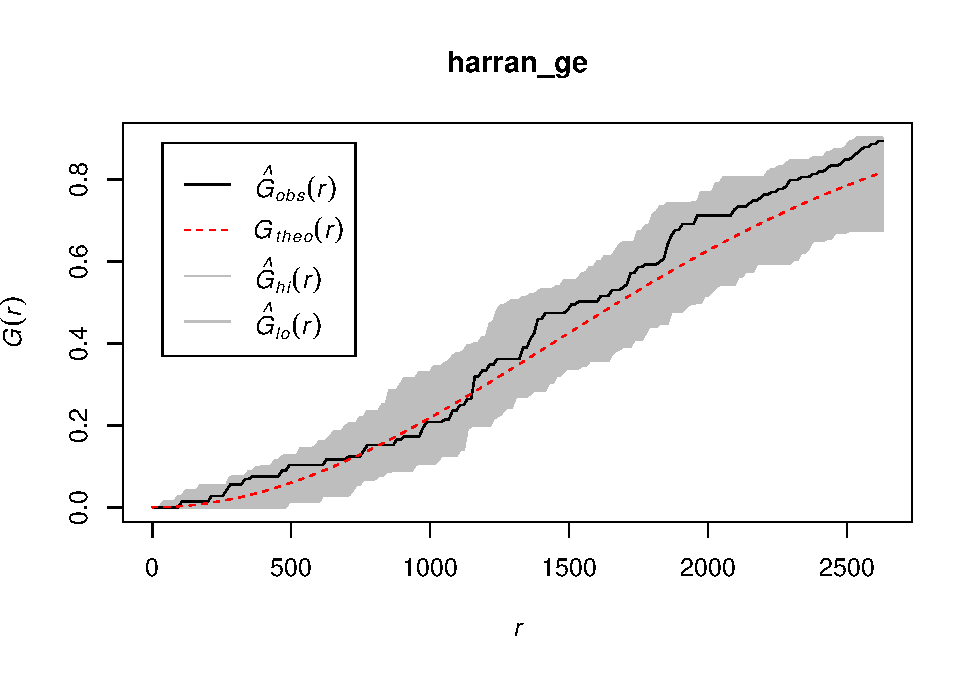
\includegraphics{HarranPlain_files/figure-latex/unnamed-chunk-9-2.pdf}

\section{challenge: do F and K
Function}\label{challenge-do-f-and-k-function}

\begin{Shaded}
\begin{Highlighting}[]
\CommentTok{#F-function:}

\NormalTok{harran_f <-}\StringTok{ }\KeywordTok{Fest}\NormalTok{(harran_ppp)}
\KeywordTok{plot}\NormalTok{(harran_f)}
\end{Highlighting}
\end{Shaded}

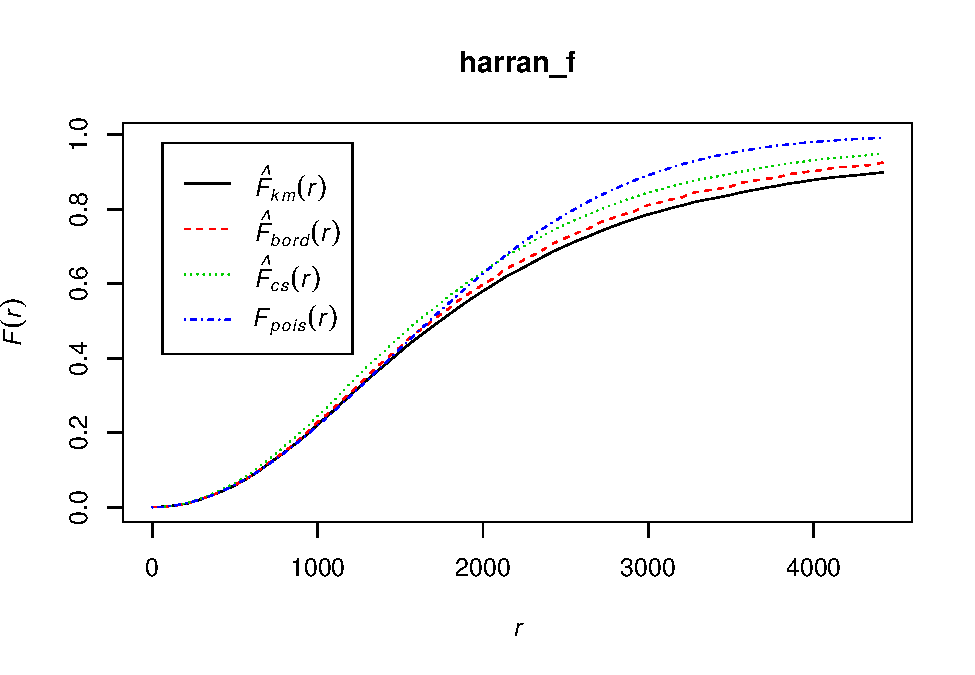
\includegraphics{HarranPlain_files/figure-latex/unnamed-chunk-10-1.pdf}

\begin{Shaded}
\begin{Highlighting}[]
\NormalTok{harran_fe <-}\StringTok{ }\KeywordTok{envelope}\NormalTok{(harran_ppp,}\DataTypeTok{fun =} \StringTok{"Fest"}\NormalTok{) }\CommentTok{# calculates f function for random points}
\end{Highlighting}
\end{Shaded}

\begin{verbatim}
## Generating 99 simulations of CSR  ...
## 1, 2, 3, 4, 5, 6, 7, 8, 9, 10, 11, 12, 13, 14, 15, 16, 17, 18, 19, 20, 21, 22, 23, 24, 25, 26, 27, 28, 29, 30, 31, 32, 33, 34, 35, 36, 37, 38,
## 39, 40, 41, 42, 43, 44, 45, 46, 47, 48, 49, 50, 51, 52, 53, 54, 55, 56, 57, 58, 59, 60, 61, 62, 63, 64, 65, 66, 67, 68, 69, 70, 71, 72, 73, 74, 75, 76,
## 77, 78, 79, 80, 81, 82, 83, 84, 85, 86, 87, 88, 89, 90, 91, 92, 93, 94, 95, 96, 97, 98,  99.
## 
## Done.
\end{verbatim}

\begin{Shaded}
\begin{Highlighting}[]
\KeywordTok{plot}\NormalTok{(harran_fe)}
\end{Highlighting}
\end{Shaded}

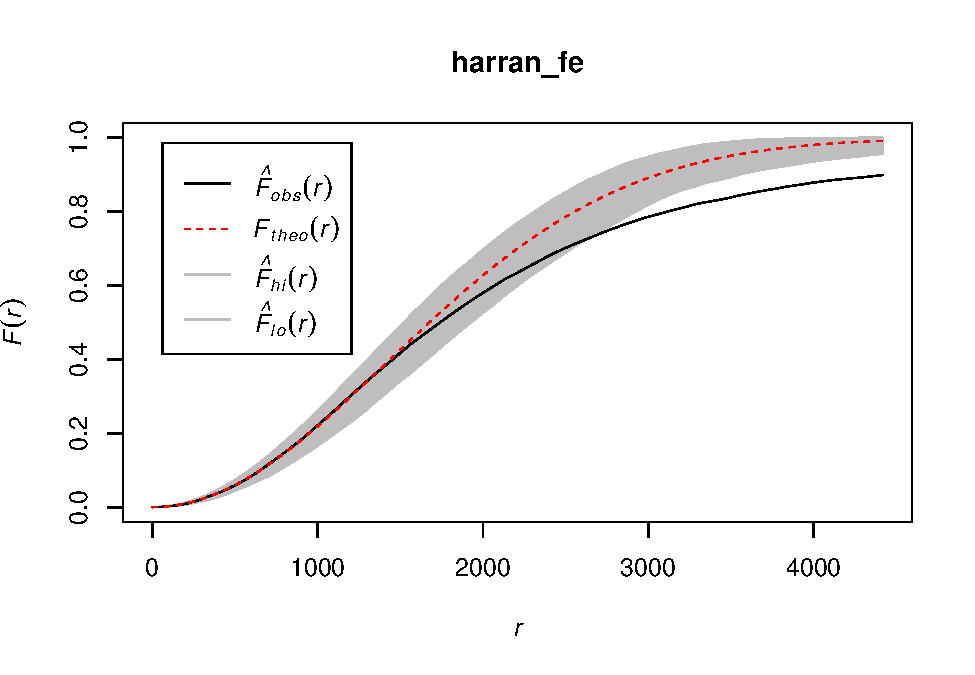
\includegraphics{HarranPlain_files/figure-latex/unnamed-chunk-10-2.pdf}

\begin{Shaded}
\begin{Highlighting}[]
\NormalTok{## red: expected, black deviates -> expect that the empty spaces are smaller than expected = clustered}


\CommentTok{#K-function}

\NormalTok{harran_k <-}\StringTok{ }\KeywordTok{Kest}\NormalTok{(harran_ppp)}
\KeywordTok{plot}\NormalTok{(harran_k)}
\end{Highlighting}
\end{Shaded}

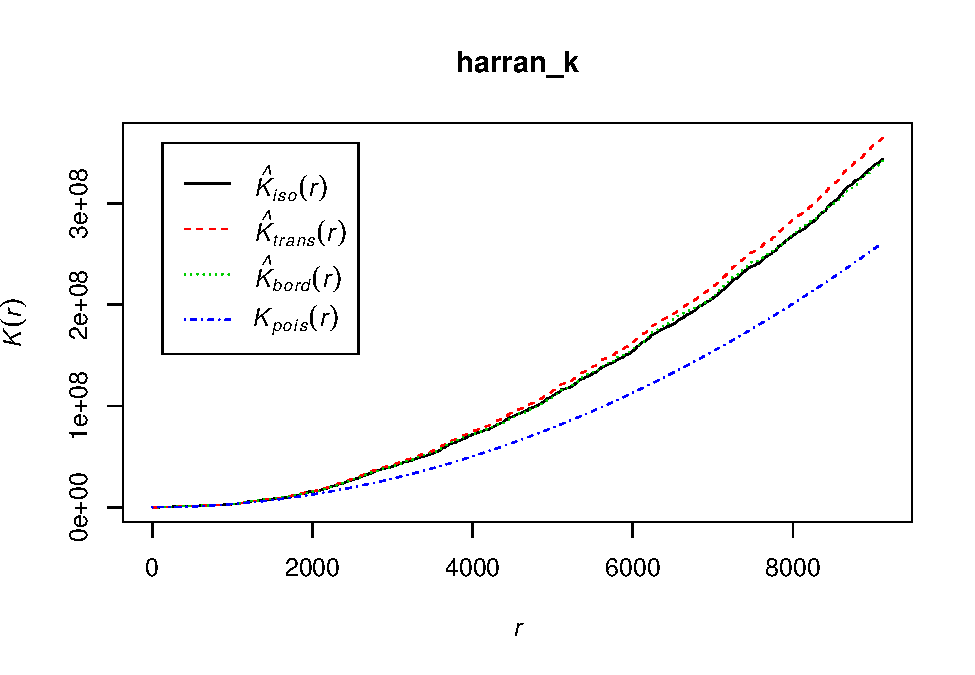
\includegraphics{HarranPlain_files/figure-latex/unnamed-chunk-10-3.pdf}

\begin{Shaded}
\begin{Highlighting}[]
\NormalTok{harran_ke <-}\StringTok{ }\KeywordTok{envelope}\NormalTok{(harran_ppp,}\DataTypeTok{fun =} \StringTok{"Kest"}\NormalTok{)}
\end{Highlighting}
\end{Shaded}

\begin{verbatim}
## Generating 99 simulations of CSR  ...
## 1, 2, 3, 4, 5, 6, 7, 8, 9, 10, 11, 12, 13, 14, 15, 16, 17, 18, 19, 20, 21, 22, 23, 24, 25, 26, 27, 28, 29, 30, 31, 32, 33, 34, 35, 36, 37, 38,
## 39, 40, 41, 42, 43, 44, 45, 46, 47, 48, 49, 50, 51, 52, 53, 54, 55, 56, 57, 58, 59, 60, 61, 62, 63, 64, 65, 66, 67, 68, 69, 70, 71, 72, 73, 74, 75, 76,
## 77, 78, 79, 80, 81, 82, 83, 84, 85, 86, 87, 88, 89, 90, 91, 92, 93, 94, 95, 96, 97, 98,  99.
## 
## Done.
\end{verbatim}

\begin{Shaded}
\begin{Highlighting}[]
\KeywordTok{plot}\NormalTok{(harran_ke) }
\end{Highlighting}
\end{Shaded}

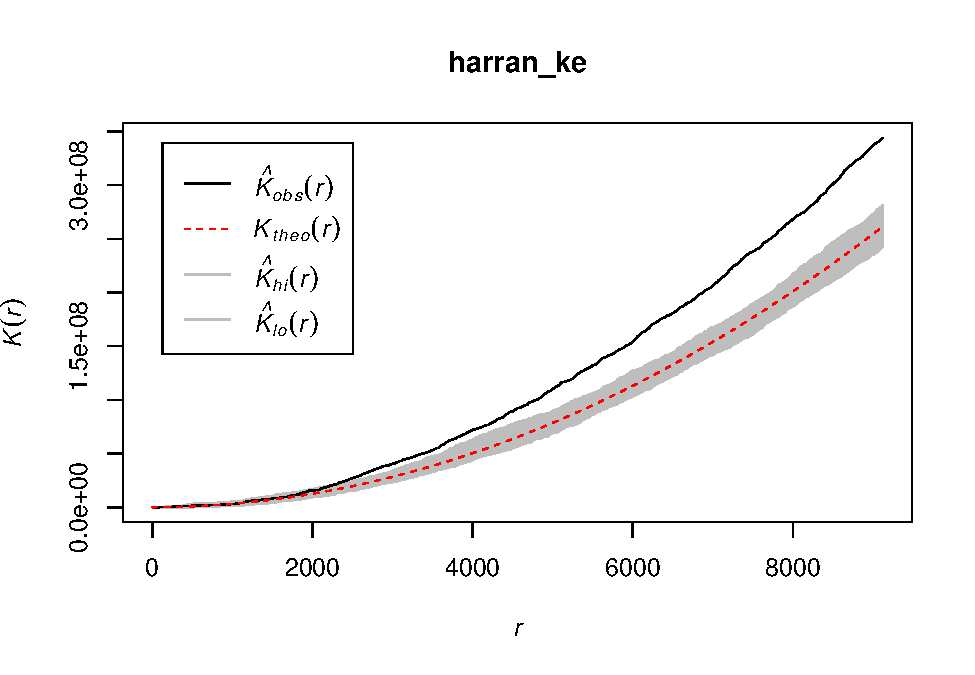
\includegraphics{HarranPlain_files/figure-latex/unnamed-chunk-10-4.pdf}

\section{Inhomogeneous Poissonfunction
G/F/K}\label{inhomogeneous-poissonfunction-gfk}

\begin{Shaded}
\begin{Highlighting}[]
\NormalTok{harran_gi <-}\StringTok{ }\KeywordTok{Ginhom}\NormalTok{(harran_ppp,}\DataTypeTok{lambda =} \KeywordTok{predict}\NormalTok{(harran_rhohat)) }\CommentTok{# harran_rhohat needs an bandwidth of 200}
\KeywordTok{plot}\NormalTok{(harran_gi)}
\end{Highlighting}
\end{Shaded}

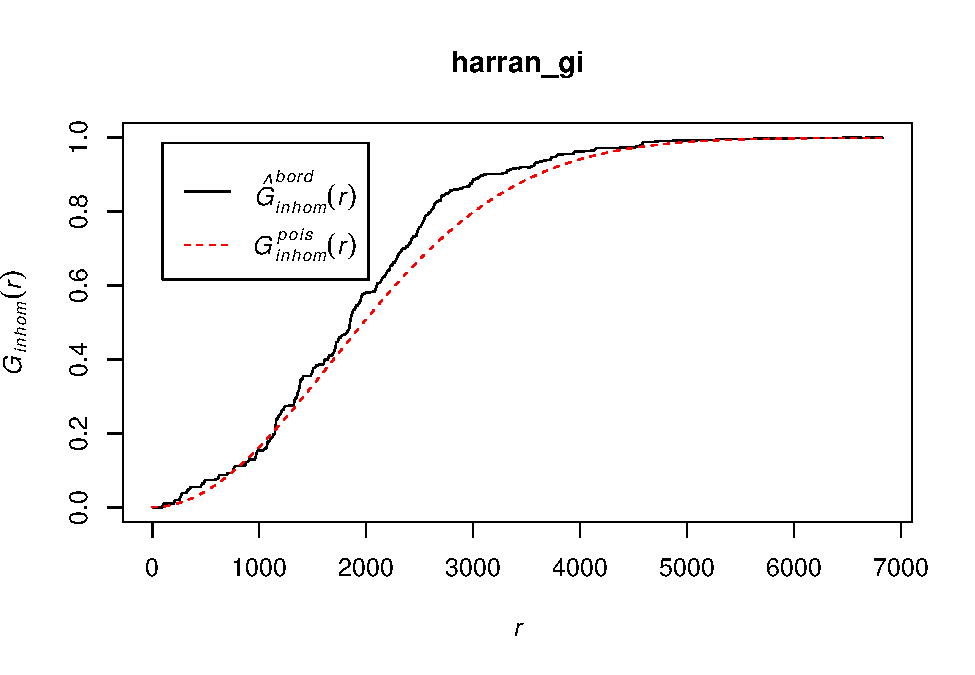
\includegraphics{HarranPlain_files/figure-latex/unnamed-chunk-11-1.pdf}

\begin{Shaded}
\begin{Highlighting}[]
\NormalTok{harran_fi <-}\StringTok{ }\KeywordTok{Finhom}\NormalTok{(harran_ppp,}\DataTypeTok{lambda =} \KeywordTok{predict}\NormalTok{(harran_rhohat))}
\KeywordTok{plot}\NormalTok{(harran_fi)}
\end{Highlighting}
\end{Shaded}

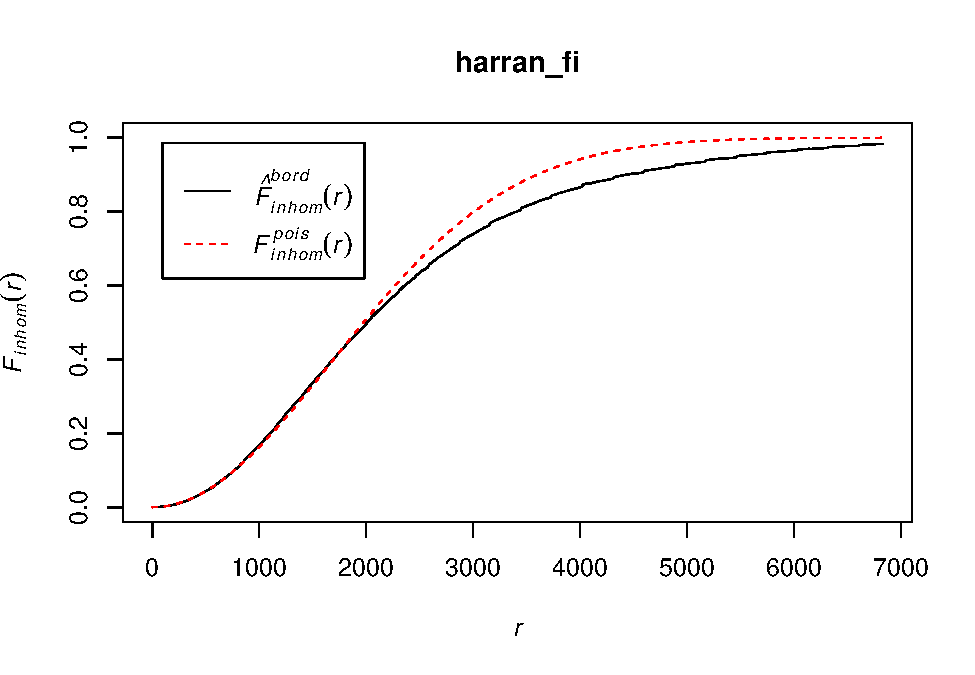
\includegraphics{HarranPlain_files/figure-latex/unnamed-chunk-11-2.pdf}

\begin{Shaded}
\begin{Highlighting}[]
\CommentTok{#par(mfrow = c(1,2))}
\CommentTok{#plot(harran_gi, xlim = c(0,6000))}
\CommentTok{#plot(harran_g, xlim = c(0,6000))      Gegenüberstellung }
\end{Highlighting}
\end{Shaded}

Note that the \texttt{echo\ =\ FALSE} parameter is added to the code
chunk to prevent printing of the R code that generated the plot.


\end{document}
